\documentclass{beamer}
\usepackage[utf8]{inputenc}

\usetheme{Madrid}
\usecolortheme{default}
\usepackage{amsmath}
\usepackage{amssymb,amsfonts,amsthm}
\usepackage{txfonts}
\usepackage{tkz-euclide}
\usepackage{listings}
\usepackage{adjustbox}
\usepackage{array}
\usepackage{tabularx}
\usepackage{gvv}
\usepackage{lmodern}
\usepackage{circuitikz}
\usepackage{tikz}
\usepackage{graphicx}

\setbeamertemplate{page number in head/foot}[totalframenumber]

\usepackage{tcolorbox}
\tcbuselibrary{minted,breakable,xparse,skins}



\definecolor{bg}{gray}{0.95}
\DeclareTCBListing{mintedbox}{O{}m!O{}}{%
  breakable=true,
  listing engine=minted,
  listing only,
  minted language=#2,
  minted style=default,
  minted options={%
    linenos,
    gobble=0,
    breaklines=true,
    breakafter=,,
    fontsize=\small,
    numbersep=8pt,
    #1},
  boxsep=0pt,
  left skip=0pt,
  right skip=0pt,
  left=25pt,
  right=0pt,
  top=3pt,
  bottom=3pt,
  arc=5pt,
  leftrule=0pt,
  rightrule=0pt,
  bottomrule=2pt,
  toprule=2pt,
  colback=bg,
  colframe=orange!70,
  enhanced,
  overlay={%
    \begin{tcbclipinterior}
    \fill[orange!20!white] (frame.south west) rectangle ([xshift=20pt]frame.north west);
    \end{tcbclipinterior}},
  #3,
}
\lstset{
    language=C,
    basicstyle=\ttfamily\small,
    keywordstyle=\color{blue},
    stringstyle=\color{orange},
    commentstyle=\color{green!60!black},
    numbers=left,
    numberstyle=\tiny\color{gray},
    breaklines=true,
    showstringspaces=false,
}
\title{3.0.25}
\date{25th March, 2026}
\author{Vishwambhar - EE25BTECH11025}

\begin{document}

\frame{\titlepage}
\begin{frame}{Question}
Let $X$ and $Y$ be two independent random variables. Which one of the relations between expectation(E), Variance(Var) and covariance (Cov) given below is FALSE?(ME 2007)\\
\begin{enumerate}
    \item $E\brak{XY}=E\brak{X}E\brak{Y}$
    \item Cov$\brak{X,Y}$ = 0
    \item Var$\brak{X+Y}=$ Var$\brak{X}+$Var$\brak{Y}$
    \item $E\brak{X^2Y^2}=\brak{E\brak{X}}^2\brak{E\brak{Y}}^2$
\end{enumerate}
\end{frame}

\begin{frame}{Definition of Independence}
$X$ and $Y$ are discrete random variables:
\begin{align}
    P(X=x,Y=y)=P(X=x)P(Y=y)
\end{align}
$X$ and $Y$ are continuous random variables:
\begin{align}
    f_{X,Y}(x,y)=f_X(x)f_Y(y)
\end{align}
\end{frame}

\begin{frame}{Option 1(Discrete)}
\begin{align}
E\brak{XY} 
&= \sum_x \sum_y xyP\brak{X=x, Y=y} \\
&= \sum_x \sum_y xyP\brak{X=x}\,P\brak{Y=y}\brak{\text{independence}} \\
&= \brak{\sum_x xP\brak{X=x}}\brak{\sum_y yP\brak{Y=y}}\\
&= E\brak{X}E\brak{Y}
\end{align}
Hence TRUE.
\end{frame}

\begin{frame}{Option 1(Continuous)}
\begin{align}
E(XY) 
&= \int_{-\infty}^{\infty} \int_{-\infty}^{\infty} xyf_{X,Y}\brak{x,y}dxdy \\
&= \int_{-\infty}^{\infty} \int_{-\infty}^{\infty} xyf_X\brak{x} f_Y\brak{y} dxdy\brak{\text{independence}} \\
&= \brak{\int_{-\infty}^{\infty} x f_X\brak{x} dx }
   \brak{\int_{-\infty}^{\infty} y f_Y\brak{y}dy}\\
&= E(X)E(Y)
\end{align}
Hence TRUE.


\end{frame}
\begin{frame}{Option 2 (Discrete, Continuous)}
\begin{align}
\text{Cov}\brak{X,Y}
&= E\brak{XY} - E\brak{X}E\brak{Y} \\
&= E\brak{X}E\brak{Y} - E\brak{X}E\brak{Y} \brak{\text{from (6) and (10)}} \\
&= 0
\end{align}
Hence TRUE.
\end{frame}

\begin{frame}{Option 3 (Discrete, Continuous)}
\begin{align}
\text{Var}\brak{X+Y}
&= E\brak{(X+Y)^2} - \brak{E\brak{X+Y}}^2 \\
&= E\brak{X^2 + Y^2 + 2XY} - \brak{E\brak{X} + E\brak{Y}}^2 \\
&= E\brak{X^2} + E\brak{Y^2} + 2E\brak{XY} - \brak{E\brak{X}^2 + E\brak{Y}^2 + 2E\brak{X}E\brak{Y}} \\
&= \brak{E\brak{X^2} - E\brak{X}^2} + \brak{E\brak{Y^2} - E\brak{Y}^2} \\
&= \text{Var}\brak{X} + \text{Var}\brak{Y}
\end{align}
Hence TRUE.
\end{frame}

\begin{frame}{Option 4 (Discrete)}
\begin{align}
E\brak{X^2Y^2}
&= \sum_x \sum_y x^2 y^2 P\brak{X=x, Y=y} \\
&= \sum_x \sum_y x^2 y^2 P\brak{X=x}P\brak{Y=y} \brak{\text{independence}} \\
&= \brak{\sum_x x^2 P\brak{X=x}}\brak{\sum_y y^2 P\brak{Y=y}} \\
&= E\brak{X^2}E\brak{Y^2}
\end{align}

But,
\begin{align}
E\brak{X^2} &= \text{Var}\brak{X} + \brak{E\brak{X}}^2 \\
E\brak{Y^2} &= \text{Var}\brak{Y} + \brak{E\brak{Y}}^2
\end{align}

\begin{align}
\Rightarrow E\brak{X^2Y^2} \neq \brak{E\brak{X}}^2 \brak{E\brak{Y}}^2
\end{align}

Hence FALSE.
\end{frame}

\begin{frame}{Option 4 (Continuous)}
\begin{align}
E\brak{X^2Y^2}
&= \int_{-\infty}^{\infty} \int_{-\infty}^{\infty} x^2 y^2 f_{X,Y}\brak{x,y} dxdy \\
&= \int_{-\infty}^{\infty} \int_{-\infty}^{\infty} x^2 y^2 f_X\brak{x} f_Y\brak{y} dxdy \brak{\text{independence}} \\
&= \brak{\int_{-\infty}^{\infty} x^2 f_X\brak{x} dx}
   \brak{\int_{-\infty}^{\infty} y^2 f_Y\brak{y} dy} \\
&= E\brak{X^2}E\brak{Y^2}
\end{align}

But,
\begin{align}
E\brak{X^2} &= \text{Var}\brak{X} + \brak{E\brak{X}}^2 \\
E\brak{Y^2} &= \text{Var}\brak{Y} + \brak{E\brak{Y}}^2
\end{align}

\begin{align}
\Rightarrow E\brak{X^2Y^2} \neq \brak{E\brak{X}}^2 \brak{E\brak{Y}}^2
\end{align}

Hence FALSE.
\end{frame}

\begin{frame}{Plot-PDF}
    \begin{figure}
        \centering
        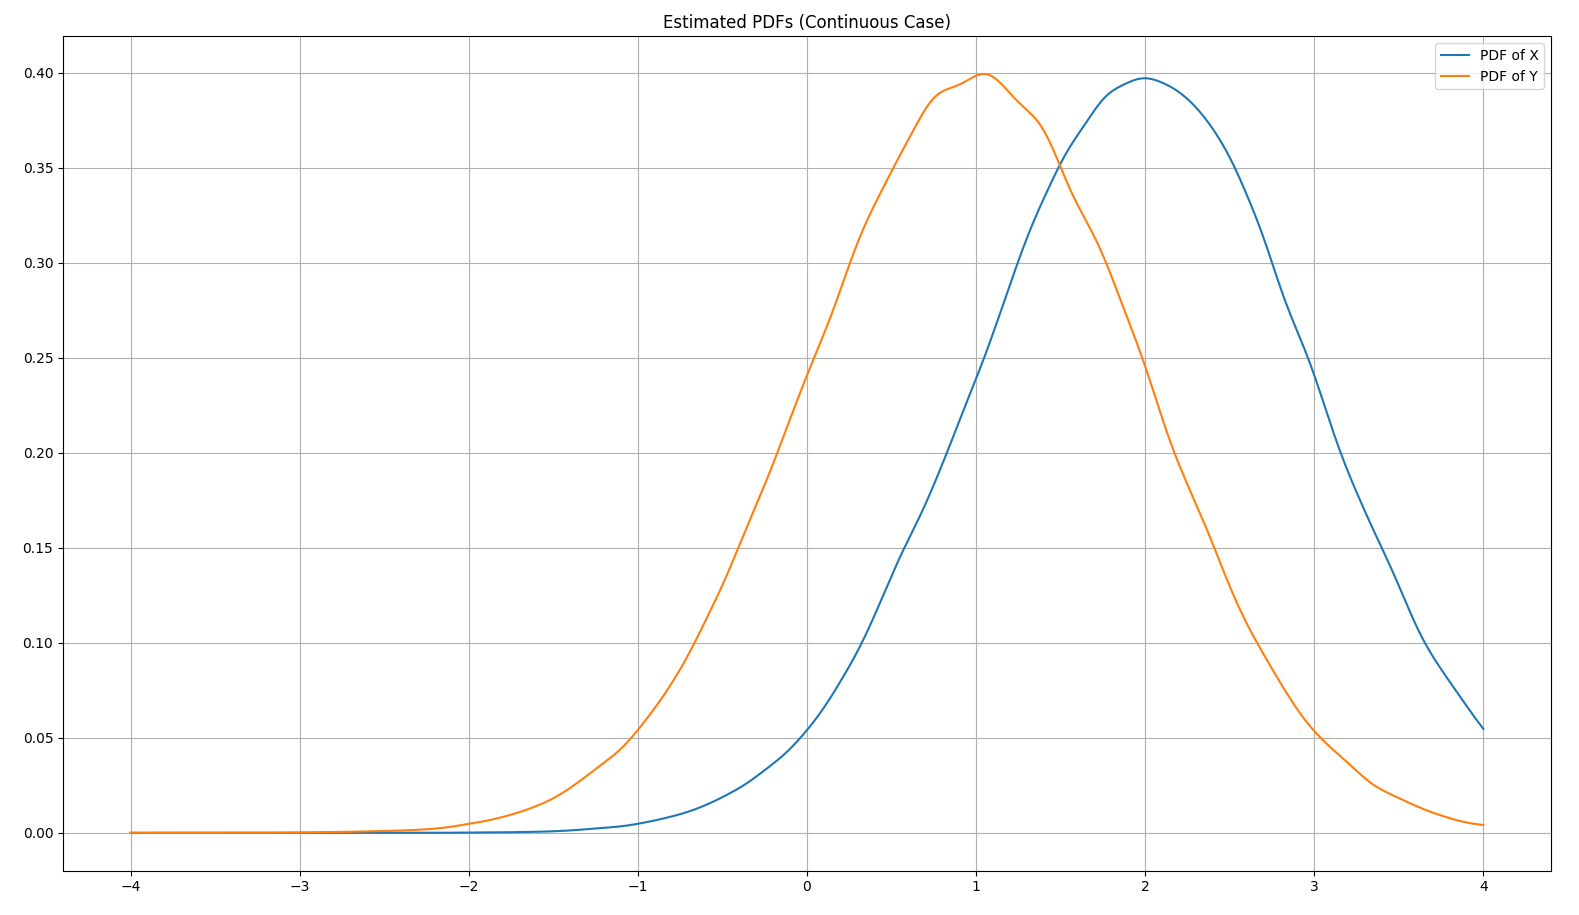
\includegraphics[width=1\columnwidth]{figs/pdf.png}
        \label{fig:fig}
    \end{figure}
\end{frame}


\begin{frame}[fragile]
    \frametitle{Python Code}
    \begin{lstlisting}
import numpy as np
import matplotlib.pyplot as plt
from scipy.stats import gaussian_kde

# Number of samples
N = 200000

def analyze(X, Y, title):
    EX = np.mean(X)
    EY = np.mean(Y)
    EXY = np.mean(X * Y)
    cov = np.mean((X - EX) * (Y - EY))
    varX = np.var(X)
    varY = np.var(Y)
    var_sum = np.var(X + Y)
    EX2Y2 = np.mean((X**2) * (Y**2))
    \end{lstlisting}
\end{frame}

\begin{frame}[fragile]
    \frametitle{Python Code}
    \begin{lstlisting}
    print(f"\n================ {title} ================")

    print("\n--- Option 1: E(XY) vs E(X)E(Y) ---")
    print(f"E(XY)        = {EXY:.2f}")
    print(f"E(X)E(Y)     = {EX * EY:.2f}")

    print("\n--- Option 2: Cov(X,Y) ---")
    print(f"Cov(X,Y)     = {cov:.2f} (should be ~0 if independent)")

    print("\n--- Option 3: Var(X+Y) vs Var(X)+Var(Y) ---")
    print(f"Var(X+Y)     = {var_sum:.2f}")
    print(f"Var(X)+Var(Y)= {varX + varY:.2f}")

    print("\n--- Option 4: E(X^2 Y^2) vs (E(X))^2 (E(Y))^2 ---")
    print(f"E(X^2 Y^2)   = {EX2Y2:.2f}")
    print(f"(E(X))^2(E(Y))^2 = {(EX**2)*(EY**2):.2f}")

    return EXY, EX*EY, cov, var_sum, varX+varY, EX2Y2, (EX**2)*(EY**2)

    \end{lstlisting}
\end{frame}

\begin{frame}[fragile]
    \frametitle{Python Code}
    \begin{lstlisting}
mux = np.random.randint(1, 5)
muy = np.random.randint(1, 5)
print(f"mux = {mux}")
print(f"muy = {muy}")
Xc = np.random.normal(mux, 1, N)
Yc = np.random.normal(muy, 1, N)
results_cont = analyze(Xc, Yc, "Continuous Case")
# KDE PDFs
kde_X = gaussian_kde(Xc)
kde_Y = gaussian_kde(Yc)
x_range = np.linspace(-4, 4, 500)
plt.figure()
plt.plot(x_range, kde_X(x_range), label="PDF of X")
plt.plot(x_range, kde_Y(x_range), label="PDF of Y")
plt.title("Estimated PDFs (Continuous Case)")
plt.legend()
plt.grid()
    \end{lstlisting}
\end{frame}

\begin{frame}[fragile]
    \frametitle{Python Code}
    \begin{lstlisting}

labels = ["Option 1", "Option 2", "Option 3", "Option 4"]

cont_vals = [
    [results_cont[0], results_cont[1]],
    [results_cont[2], 0],
    [results_cont[3], results_cont[4]],
    [results_cont[5], results_cont[6]]
]

plt.figure()
for i in range(4):
    plt.scatter([i, i], cont_vals[i])
plt.xticks(range(4), labels)
plt.title("Continuous Case Verification")
plt.grid()

plt.show()
    \end{lstlisting}
\end{frame}

\begin{frame}{Results}
    \begin{figure}
        \centering
        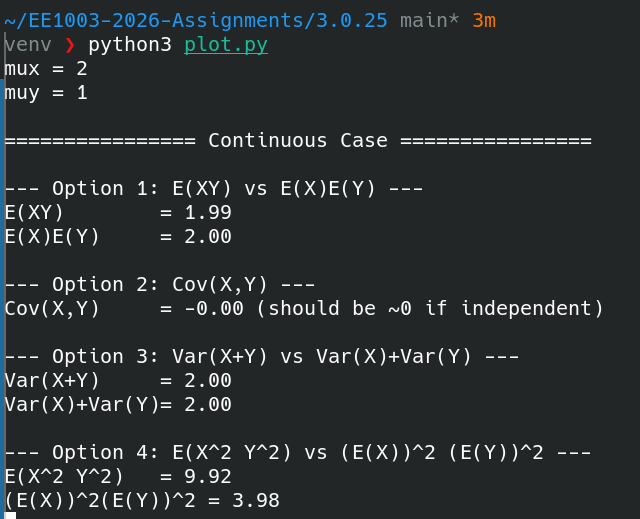
\includegraphics[width=0.6\columnwidth]{figs/Results.png}
        \label{fig:fig}
    \end{figure}
\end{frame}

\end{document}